\documentclass{article}
\usepackage{geometry}
\usepackage{hyperref}
\usepackage{graphicx}

\title{System Architecture Document}
\date{\today}

\begin{document}

\maketitle

\section{Architectural design strategy}

\subsection{Background}
For our logistics optimization system, we aimed to develop a comprehensive solution that addresses the unique needs of managing and optimizing the placement of goods in logistics trucks. Our system leverages dynamic algorithms and machine learning models to enhance efficiency and space management. This application will assist logistics managers in predicting office capacities and managing desk allocations to prevent overbooking. Given the diverse and demanding requirements of such a system, we have focused on ensuring high performance, scalability, security, reliability, and usability.

\subsection{Architectural Decisions}
The architectural decisions have been based on the quality requirements of the system. We have used the quality requirements (listed in our System Requirements Specification: SRS) to identify our quality requirements which were used to identify our architectural patterns.

\section{Architectural quality requirements}

\textbf{Performance:}
\begin{itemize}
    \item The application shall have fast response times for user interactions.
    \item The application's database operations, implemented with Supabase, should have efficient query execution times to ensure quick retrieval and storage of data.
    \item The system should return the optimal packing route within 2-5 minutes of the provided configuration/input parameters.
    \item The real-time 3D render should reflect optimizations in real time without any delay or buffering.
\end{itemize}

\textbf{Scalability:}
\begin{itemize}
    \item The backend infrastructure, particularly the database layer hosted on Supabase, should be capable of handling increasing loads as the user base expands.
    \item The system should be scalable in the sense the algorithm could potentially be used for packing cargo trains, or shipping containers.
\end{itemize}

\textbf{Security:}
\begin{itemize}
    \item All user authentication and authorization processes, including registration, login, and password reset, must follow the best practices for safe transfer and storage of sensitive user information.
    \item Data stored in the Supabase database must be encrypted to protect user privacy and comply with relevant data protection regulations.
\end{itemize}

\textbf{Reliability:}
\begin{itemize}
    \item Error handling mechanisms shall be implemented to handle erroneous input and provide helpful feedback to users in case of unexpected errors.
    \item Continuous integration and deployment pipelines (CI/CD) shall be set up using GitHub Actions to ensure reliable software releases.
\end{itemize}

\textbf{Usability:}
\begin{itemize}
    \item The application shall have an intuitive and user-friendly interface to ensure ease of use for all user types, including logistics managers, truck drivers, and warehouse staff.
    \item The interface should be accessible and provide a consistent user experience across various devices and screen sizes.
    \item The system shall provide clear instructions and feedback to users, guiding them through the process and informing them of any errors or required actions.
    \item The system shall provide real-time updates to users, ensuring they are always informed of the current status and any changes in the packing process.
\end{itemize}

\section{Architectural Strategies}
The Extended Planning Instrument for Unpredictable Spaces and Environment is coupled with the following architectural patterns; layered, API gateway, and service-oriented architecture of the software. The different architectural patterns are shown in the following diagram:

\begin{figure}[h]
    \centering
    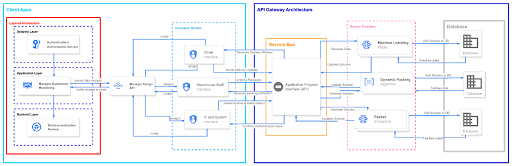
\includegraphics[width=\textwidth]{architecturalDiagram.png}
    \caption{Architecture Diagram}
    \label{fig:arch_diagram}
\end{figure}

\end{document}
